% 建议使用 XeLaTeX 或 LuaLaTeX 编译(中文与公式支持更佳)
\documentclass[UTF8,zihao=-4]{ctexart}

\usepackage[a4paper,margin=2.5cm]{geometry}
\usepackage{amsmath, amssymb, amsthm}
\usepackage{bm}
\usepackage{hyperref}
\usepackage{graphicx}
\usepackage{caption}
\usepackage{listings}
\usepackage{xcolor}
\usepackage{float}
\usepackage{placeins}
\graphicspath{{figures/}}

\lstdefinestyle{code}{
  basicstyle=\ttfamily\small,
  numbers=left,
  numberstyle=\tiny,
  numbersep=8pt,
  keywordstyle=\color{blue},
  commentstyle=\color{teal!70!black},
  stringstyle=\color{orange!70!black},
  showstringspaces=false,
  breaklines=true,
  frame=single,
  framerule=0.3pt,
  rulecolor=\color{black!15}
}
\lstset{style=code}

\title{Isolation Forest 异常检测:原理、公式、应用与实战}
\author{}
\date{\today}

\begin{document}
\maketitle

\section{引言}
Isolation Forest 通过随机划分样本直至其被孤立来识别异常点。与基于密度的算法不同,它利用异常样本在特征空间中稀疏、偏离正常簇这一事实:异常越孤立,越容易被分割到独立节点,从而得到高的异常分数。

\section{原理与公式}
\subsection{随机划分}
每棵隔离树(isolation tree)通过随机选择特征并在该特征范围内随机生成分割值来递归划分样本。样本 \(\mathbf{x}\) 的路径长度 \(h(\mathbf{x})\) 指从根节点到叶节点的分割次数。异常点通常在更短路径上被隔离,而正常点则需要更多分割。

\subsection{路径长度与异常分数}
若子样本量为 \(\psi\),二叉搜索树未成功搜索的期望路径长度为
\begin{equation}
\mathbb{E}[h(\psi)] = 2 H_{\psi-1} - \frac{2(\psi-1)}{\psi}, \qquad H_n = \sum_{k=1}^n \frac{1}{k}.
\end{equation}
Isolation Forest 的异常分数定义为
\begin{equation}
s(\mathbf{x}, \psi) = 2^{-\frac{\overline{h(\mathbf{x})}}{\mathbb{E}[h(\psi)]}},
\end{equation}
其中 \(\overline{h(\mathbf{x})}\) 为多棵树的平均路径长度。分数接近 1 表示强烈异常,低于 0.5 通常视为正常。

\subsection{超参数与复杂度}
主要参数包括树的数量、子样本大小以及用于设定阈值的污染率(contamination)。Isolation Forest 对 \(t\) 棵树、子样本大小 \(\psi\) 的时间复杂度约为 \(O(t \psi \log \psi)\),具备线性扩展性。特征缩放、处理类别变量以及合理设定污染率对模型性能尤为重要。

\section{应用与技巧}
\begin{itemize}
  \item \textbf{欺诈检测}:发现金融或电商中极不寻常的交易。
  \item \textbf{网络安全}:定位高维日志中的罕见流量模式或攻击迹象。
  \item \textbf{工业监控}:识别偏离正常运行状态的传感器读数。
  \item \textbf{实用建议}:对特征做标准化,调节子样本大小与污染率,分析分数分布,并结合领域知识确认告警的合理性。
\end{itemize}

\section{Python 实战}
脚本 \texttt{gen\_isolation\_forest\_figures.py} 构造含噪声的数据集,训练 scikit-learn 的 IsolationForest,并可视化特征空间中的异常分布以及分数直方图。
\begin{lstlisting}[language=Python,caption={脚本 gen_isolation_forest_figures.py 片段}]
from sklearn.ensemble import IsolationForest

model = IsolationForest(
    n_estimators=200,
    max_samples=256,
    contamination=0.08,
    random_state=42,
)
model.fit(points)
score = model.decision_function(points)
labels = model.predict(points)
\end{lstlisting}

\section{实验结果}
\begin{figure}[H]
  \centering
  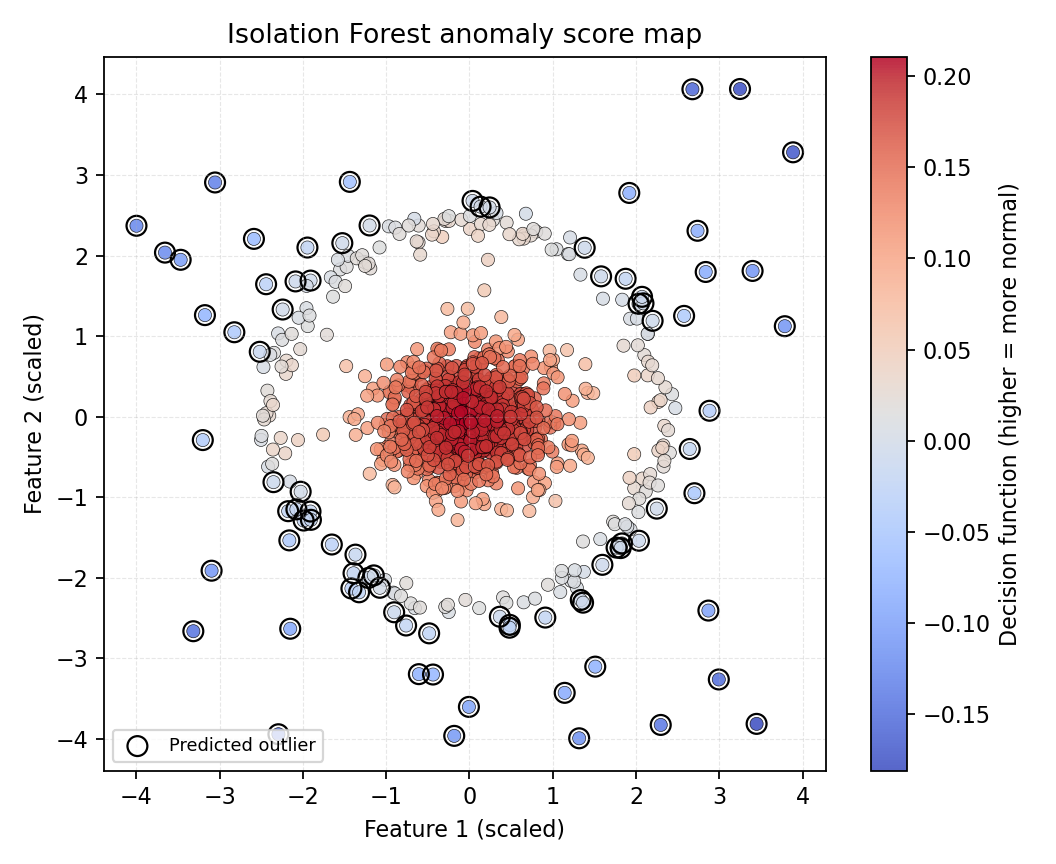
\includegraphics[width=0.82\linewidth]{isolation_forest_decision.png}
  \caption{Isolation Forest 在模拟数据上的异常分数热度图,颜色越深表示越异常}
  \label{fig:isolation_forest_decision_cn}
\end{figure}

\begin{figure}[H]
  \centering
  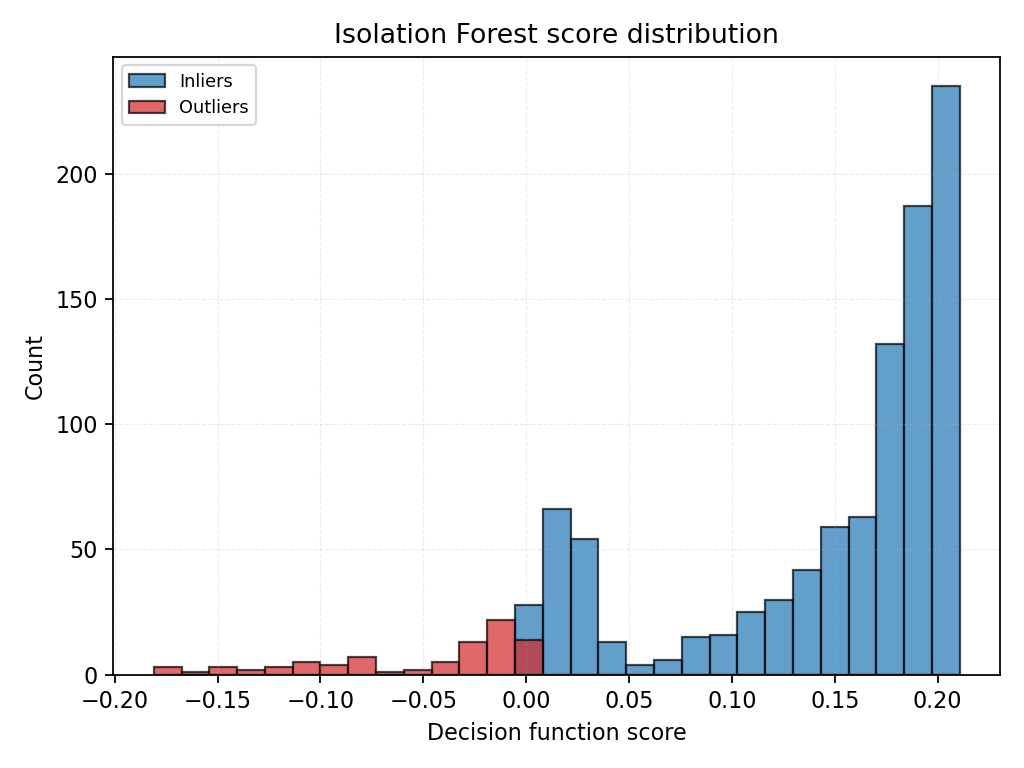
\includegraphics[width=0.78\linewidth]{isolation_forest_score_hist.png}
  \caption{异常分数直方图,对比模型判定的正常与异常样本}
  \label{fig:isolation_forest_score_hist_cn}
\end{figure}

\FloatBarrier
\section{总结}
Isolation Forest 通过随机分割高效孤立异常点,适用于高维、少假设的场景。只要结合特征缩放与参数调优,并对分数结果进行可视化检查,就能在实际业务中取得稳定的异常检测效果。示例展示了如何基于分数图与直方图评估阈值选择及异常分布。

\end{document}